% 单色光

可见光是波长在$400-760\mathrm{nm}$,亦即频率在$4.3 \times 10^{14} \sim 7.5 \times 10^{14} \mathrm{Hz}$之间的电磁波.具有单一频率的光波称为单色光(monochromatic light).然而,严格的单色光是不存在的.任何光源所发出的光波都有一定的频率(或波长)范围,在此范围内,各种频率(或波长)所对应的强度是不同的,以波长为横坐标,强度为纵坐标,可以直观地表示出这种强度与波长间的关系,称为\textbf{光谱曲线},或称\textbf{谱线(spectrum)},如\autoref{MonoLi_fig1}所示,谱线所对应的波长范围越窄,则称光的单色性越好.
\begin{figure}[ht]
\centering
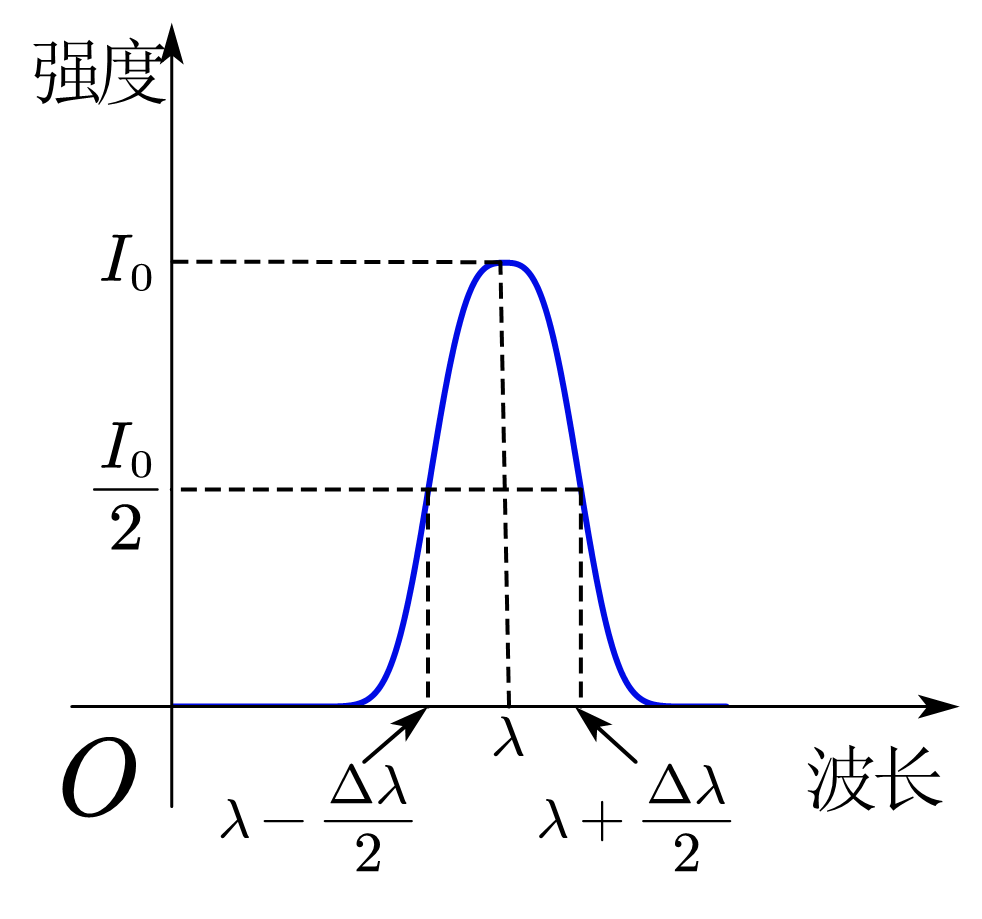
\includegraphics[width=5cm]{./figures/MonoLi_1.png}
\caption{谱线及其宽度} \label{MonoLi_fig1}
\end{figure}

设谱线中心处的波长为$\lambda$,强度为$I_0$,通常用最大强度的一半所包围的波长范围$\Delta\lambda$当作\textbf{谱线宽度}(line width),它是标志谱线单色性好坏的物理量.普通单色光源,如钠光灯、镉灯、汞灯等,谱线宽度的数量级为$0.1 \sim 10^{-3} \mathrm{nm}$,而激光的谱线宽度只有$10^{-9}\mathrm{nm}$,甚至更小.
